% Author: Izaak Neutelings (September 2021)
% Inspiration:
%   https://jila.colorado.edu/~ajsh/insidebh/penrose.html
%   https://tex.stackexchange.com/questions/99124/how-to-draw-penrose-diagrams-with-tikz
%   coordinates: https://arxiv.org/pdf/physics/0611033.pdf
%   https://arxiv.org/pdf/0711.0873.pdf

\documentclass[border=3pt,tikz]{standalone}
\usepackage{tikz}
\usepackage{amsmath}
\usepackage{mathrsfs}
\usepackage{xfp}
\usepackage[outline]{contour}
\usetikzlibrary{decorations.pathmorphing}
\contourlength{1.4pt}

\newcommand{\calI}{\mathscr{I}}

\colorlet{myred}{red!80!black}
\colorlet{myblue}{blue!80!black}
\colorlet{mydarkblue}{blue!50!black}
\colorlet{mylightblue}{mydarkblue!6}
\colorlet{mypurple}{blue!40!red!80!black}
\colorlet{mydarkpurple}{blue!40!red!50!black}
\colorlet{mylightpurple}{mydarkpurple!80!red!6}

\tikzstyle{world line}=[myblue!60,line width=0.4]
\tikzstyle{world line t}=[mypurple!60,line width=0.4]
\tikzstyle{singularity}=[myred,line width=0.6,decorate,
                         decoration={zigzag,amplitude=2,segment length=6.17}]

\tikzset{declare function={%
  kruskal(\x,\c) = {\fpeval{asin( \c*sin(2*\x) )*2/pi}};%
}}

\def\Nsamples{40}

\begin{document}

% Diagramme de Penrose sch\'ematique : trou noir charg\'e en relativit\'e intriqu\'ee
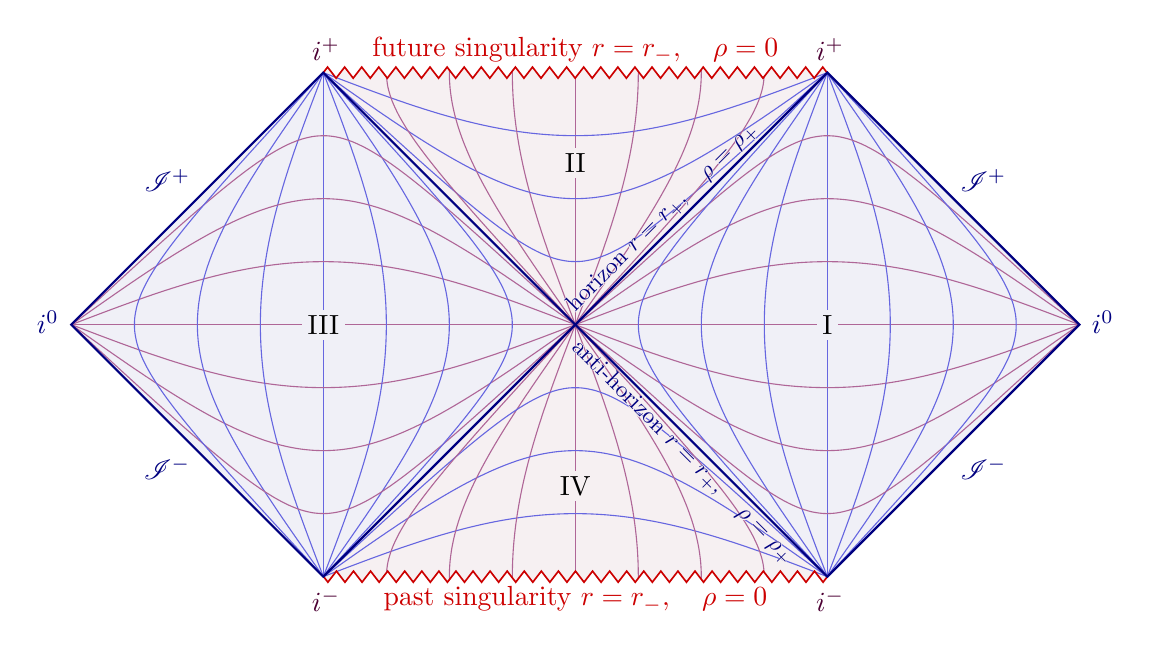
\begin{tikzpicture}[scale=3.2]

  \def\Nlines{3}

  % Coordonnees principales
  \coordinate (-O) at (-1, 0);
  \coordinate (-S) at (-1,-1);
  \coordinate (-N) at (-1, 1);
  \coordinate (-W) at (-2, 0);
  \coordinate (-E) at ( 0, 0);
  \coordinate (O)  at ( 1, 0);
  \coordinate (S)  at ( 1,-1);
  \coordinate (N)  at ( 1, 1);
  \coordinate (E)  at ( 2, 0);
  \coordinate (W)  at ( 0, 0);

  \begin{scope}

    % Coupure au niveau des singularites en zigzag
    \clip[decorate,decoration={zigzag,amplitude=2,segment length=6.17}]
      (S) -- (-S) --++ (-1.1,-0.1) |-++ (4.2,2.2) |- cycle;
    \clip[decorate,decoration={zigzag,amplitude=2,segment length=6.17}]
      (-N) -- (N) --++ (1.1,0.1) |-++ (-4.2,-2.2) |- cycle;

    % Remplissage des regions
    \fill[mylightpurple] (-N) |-++ (2,0.1) -- (N) -- (-S) -- (S) -- cycle;
    \fill[mylightpurple] (-S) |-++ (2,-0.1) -- (S) -- (-N) -- (N) -- cycle;
    \fill[mylightblue] (-N) -- (-E) -- (-S) -- (-W) -- cycle;
    \fill[mylightblue] (N) -- (E) -- (S) -- (W) -- cycle;

    % Lignes de coordonnees conformes
    \draw[world line] (-N) -- (-S) (N) -- (S);
    \draw[world line t] (-W) -- (-E) (W) -- (E) (0,-1.1) -- (0,1.1);

    \foreach \i [evaluate={\c=\i/(\Nlines+1); \cs=sin(90*\c);}] in {1,...,\Nlines}{
      \draw[world line t,samples=2*\Nsamples,smooth,variable=\x,domain=-2:2]
        plot(\x,{-kruskal(\x*pi/4,\cs)})
        plot(\x,{ kruskal(\x*pi/4,\cs)});

      \draw[world line,samples=\Nsamples,smooth,variable=\y,domain=0:2]
        plot({-1-kruskal(\y*pi/4,\cs)},\y-1)
        plot({-1+kruskal(\y*pi/4,\cs)},\y-1)
        plot({ 1-kruskal(\y*pi/4,\cs)},\y-1)
        plot({ 1+kruskal(\y*pi/4,\cs)},\y-1);

      \draw[world line,samples=\Nsamples,smooth,variable=\x,domain=0:2]
        plot(\x-1,{kruskal(\x*pi/4,\cs)-1})
        plot(\x-1,{1-kruskal(\x*pi/4,\cs)});

      \draw[world line t,samples=\Nsamples,smooth,variable=\y,domain=-1.05:1.05]
        plot({-kruskal(\y*pi/4,\cs)},\y)
        plot({ kruskal(\y*pi/4,\cs)},\y);
    }

  \end{scope}

  % Singularites
  \draw[singularity] (-N) -- node[above] {future singularity $r=r_-,\ \ \ \rho = 0$} (N);
  \draw[singularity] (S) -- node[below] {past singularity $r=r_-,\ \ \ \rho = 0$} (-S);

  % Horizons
  \path (S) -- (W) node[mydarkblue,pos=0.52,below=-2.5,rotate=-45,scale=0.85]
    {\contour{mylightpurple}{anti-horizon $r=r_+,\ \ \ \rho = \rho_+$}};
  \path (W) -- (N) node[mydarkblue,pos=0.40,above=-2.5,rotate=45,scale=0.85]
    {\contour{mylightpurple}{horizon $r=r_+,\ \ \ \rho = \rho_+$}};

  % Frontieres conformes
  \draw[thick,mydarkblue] (-N) -- (-E) -- (-S) -- (-W) -- cycle;
  \draw[thick,mydarkblue] (N) -- (E) -- (S) -- (W) -- cycle;

  % Regions
  \node[fill=mylightblue,inner sep=2] at (-O) {III};
  \node[fill=mylightblue,inner sep=2] at (O) {I};
  \node[fill=mylightpurple,inner sep=2] at (0,0.64) {II};
  \node[fill=mylightpurple,inner sep=2] at (0,-0.64) {IV};

  % Infinis conformes
  \node[above=1,left=1,mydarkblue] at (-2,0) {$i^0$};
  \node[above=1,right=1,mydarkblue] at (2,0) {$i^0$};
  \node[right=1,below=1,mydarkpurple] at (-S) {$i^-$};
  \node[right=1,above=1,mydarkpurple] at (-N) {$i^+$};
  \node[right=1,below=1,mydarkpurple] at (S) {$i^-$};
  \node[right=1,above=1,mydarkpurple] at (N) {$i^+$};
  \node[mydarkblue,below left=-1] at (-1.5,-0.5) {$\calI^-$};
  \node[mydarkblue,above left=-1] at (-1.5,0.5) {$\calI^+$};
  \node[mydarkblue,above right=-1] at (1.5,0.5) {$\calI^+$};
  \node[mydarkblue,below right=-1] at (1.5,-0.5) {$\calI^-$};

\end{tikzpicture}

\end{document}